\subsection{EMT Design}
\label{emt:sec:design}

\noindent
Extensible Memory Translation (EMT) is an OS framework
	built atop Linux
	with the goal of empowering new, experimental memory translation architectures.
% In this section, we discuss the OS framework;
%	we discuss our emulator-based toolchains for 
%	developing and evaluating experimental translation
%	architectures like ECPT in \S\ref{emt:sec:ecpt_impl}.
Figure~\ref{emt:fig:emt-overview} gives a high-level overview of EMT.
% We target Linux % , instead of more extensible OS kernels (e.g., microkernels~\cite{krueger1993tools}
%	% and exokernels~\cite{engler1995avm})
%	as it is still the {\it de facto} commodity OS for memory-intensive computing
%	and assumed by most architecture research on memory systems.
EMT currently focuses on supporting new memory translation architectures in the OS kernel, instead of
	exposing them to userspace~\cite{engler1995avm}.
The design and implementation of EMT achieves the following goals:
\begin{packed_itemize}%[\labelitemi]
\item{\bf EMT is an architecture-neutral framework.}
EMT is not hardwired to specific translation structures such as
	multi-level tree in Linux.
% As discussed in \S\ref{emt:sec:need:hardwire},
%	hardwired designs are fundamentally limited in extensibility.
%In principle, s
Supporting a new memory translation scheme should not change % effectively reuse
	architecture-independent code.
% - Decoupled, Clear semantics, Support diverse memory translations, extensibility.
% With the interface, memory translation developers
% only need to implement an \mmudriver corresponding to their translation hardware to make the kernel
% support it. \interface guides them by providing the full list of required driver
% functions.

\item{\bf EMT enables hardware-specific optimizations.}
% EMT exposes architecture-neutral primitives 
%	to OS memory management 
EMT allows architecture-dependent code 
	to customize routines for hardware-specific optimizations.
	The ability to customize differs EMT from high-level interfaces like pmap in Mach/BSD~\cite{rashid1987machine}
	and hat in SunOS~\cite{gingell1987sunos}.
% A key challenge is to devise translation primitives that are essential to 
%	optimizations and are architecture neutral.
% - MMU driver, EMT interface, generic interface, optimizability,
% comprehensiveness.
% - Essential groups and Optimization groups.

% \interface is composed of generic functions that is shared by different memory
% translation architectures. It is enough to use the generic functions for the
% functionality. However, memory translation developers would want to improve the
% performance by applying architecture-specific optimizations to the kernel stack.
% \interface provides an option to register architecture-specific functions to
% satisfy the needs (\optgrps in Figure \ref{emt:figure:interface-internal}).

\item{\bf EMT is modularized and improves maintainability.}
EMT provides well-defined translation semantics and organizes them with an object-oriented design.
%	(in a similar vein to VFS~\cite{linux:vfs}).
The interface eliminates architecture-specific or overloaded semantics. % (\S\ref{emt:sec:need:hardwire}).
EMT also makes it easy to profile and analyze OS performance with regard to translation architectures.
%	by capturing memory management operations related to translation.

% EMT can be adopted to the kernel simply by replacing corresponding functions in its callers
% with the \interface functions. 
% \jyk{Is it true?} 
% \JZc{largely, but not always - for example we need to replace loops to iterator pattern}

\item{\bf EMT has negligible overhead.}
% - Macro and inline function
% - Compatible to the existing kernel.
% Memory management operations are performance critical~\cite{yan2019nimble,huang16mmstudy}.
% EMT avoids introducing new OS abstractions.
EMT is 
% \jzx{extensively optimized}{
	carefully implemented with
%	\jzx{inline functions and macros, and has 
%	negligible overhead (\S\ref{emt:sec:eval:eval-EMT-radix-vs-vanilla}).}{
	compiler optimization, cache efficiency, and the ability to inline functions.
EMT-Linux serves as a performance baseline for 
	new architectures or OS modules.

\item{\bf EMT accommodates modern hardware and OS complexity.}
EMT aims to develop insights into complex OS-architecture interactions.
% EMT is not designed to merely serve as a benchmark runner, rather, it should also help researchers validate their design against known use cases,
%	so it can help users expose and resolve problems in designs as early as possible.
EMT supports {\it all} Linux's memory management features related to CPU MMU % related to memory translation.
	translation such as huge pages, swapping, DAX memory, etc.
%	such as page fault handling, KPTI~\cite{linux:kpti}, THP~\cite{linux:thp}, context switch, etc.

\end{packed_itemize}

\begin{figure}[H]
	\centering
	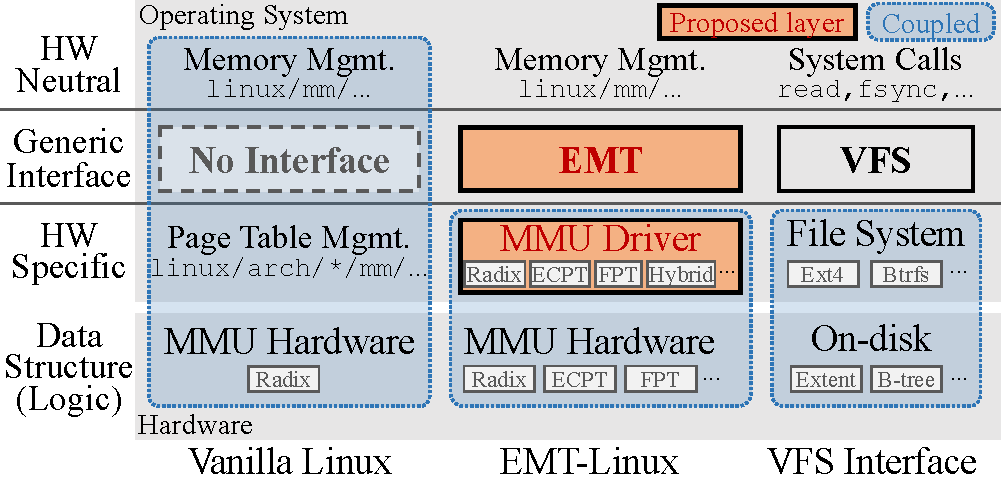
\includegraphics[width=0.475\textwidth]{figs/interface_overview.pdf}
	% \vspace*{-7mm}
%	\captionsetup{justification=centering}
%	\caption{{\bf Linux with \branding and an analogy with the
%		VFS interface~\cite{linux:vfs}.} \branding decouples the
%		architecture-neutral layer from hardware whereas it is coupled
%		in vanilla Linux.}
%		\label{emt:figure:interface-overview}
\caption{\bf Overview of the EMT framework, compared with vanilla Linux
	and analogized to VFS.}
	% \jyk{I modified some names. Is there anthing else you want to change?}}
	\label{emt:fig:emt-overview}
\end{figure}

\subsubsection{EMT API}

% EMT interface
% \interface is a generic interface that is independent from the hardware
% implementation of memory translations.

\noindent
EMT exposes an object-oriented API that organizes translation related 
	kernel routines around three architecture-neutral
primitives:
% \begin{packed_itemize}%[\labelitemi]
1)	{\it translation object} that maintains all the information of 
	a virtual-to-physical address translation,
%	for a virtual address, including
%	 virtual-to-physical address mapping 
%	and its metadata,
2) {\it translation database} that stores translation objects
	of an address space, 
and 3) {\it translation service} that manages the MMU states. % and its states.
%	(a process may has multiple context).
%	(associated database(s) and control registers).
	% \TODO{TODO: I don't know what it is for now;
	%	will write after I know more.}
% \end{packed_itemize}

In EMT, all architecture-dependent code is implemented in drivers 
	for MMU architectures,
	referred to as {\it MMU drivers}.
To support a new translation scheme on EMT-Linux,
	one needs to write the MMU driver that implements EMT API
	\schai{without the need to modify architecture-independent code}.


A key design principle of
	the EMT API is to abstract the {\it functions} of translation
	for OS memory management from hardware-defined {\it shapes}.
Despite many different translation architectures (\S\ref{emt:sec:background}),
	the essential function of memory translation is to output the virtual-to-physical
	address mapping and all associated metadata, which is abstracted 
	as a {\it translation object} in EMT.
EMT avoids assuming shapes
	of translation data like translation entry schema
	or translation data structures.
How to encode translation information 
	of hardware-defined shapes into the EMT API is the job of MMU drivers.
% This API design fundamentally differs from existing Linux 
%	routines hardwired 
%	to the \textit{shape} of translation data (\S\ref{emt:sec:need}).

% the translation entry or the granularity of the mapping 
%	(e.g., for different page sizes).
% EMT does {\it not} assume the shape of the translation database (a linear array,
%	a radix tree, or a hash table).

%The three objects are neutral to 
%	% the minimal set of abstractions that are not specific to any 
%	different translation architectures,
%	and are sufficient to express all the historical, current,
%	and recently proposed translation architectures (\S\ref{emt:sec:design:generality}).
The EMT API is organized as 
	1) {\it basic functions} that must be implemented by each MMU driver
	for its supporting translation architecture,
% to allow the system to function properly (Figure~\ref{emt:fig:emt-overview}).
	and 2) {\it customizable functions} that have a default implementation
	that is architecture-independent; the default implementation 
	only uses basic functions and other common code. % is architecture-neutral.
	These routines can be customized by MMU drivers 
	for hardware-specific optimizations.

\schai{The basic functions represent the 
	minimal set of functions to support a new translation architecture. 
Developers can start with basic functions to achieve a functional kernel 
	and then iteratively add optimizations via customizable functions.
Basic functions free developers from sophisticated optimizations 
	in Linux; 
	it leads to a more friendly development and test cycle.}

% These routines cover low-level primitives 
%	that are commonly referenced in optimizations 
%	of OS memory management code.
% Specifically:
% \begin{packed_itemize}%[\labelitemi]
%	\item {\bf basic functions} are kernel routines
%	that must be implemented
%		for each supported translation architecture in the architecture-dependent 
%		code to allow the system to function properly (Figure~\ref{emt:fig:emt-overview}).
%		In other words, they represent the minimal effort to implement 
%		in order to support a new translation architecture.
%	\item {\bf customizable functions} are kernel routines that have default implementation
%		in architecture-independent code; the default implementation 
%		only uses basic functions and thus is architecture-neutral.
%		However, these routines can be customized for architecture-specific optimizations.
%		\TODO{Specifically, we identify \TODO{XXX} abstractions 
%			such as locks, iterators, and \TODO{XXX}
%			whose customization often leads to major performance improvements}.
%		We show in \S\ref{emt:sec:todo} that customizing some of them leads to 
%		significant performance benefits.
% \end{packed_itemize}

% \TODO{do we need this? it may help.}
% The driver will be compiled as a part of the EMT-Linux kernel binary.
% \TODO{4.1 reads rather boring. Can we think about what insights to put here?}

%TODO: Do we need to describe more details such as generic functions and registering file
%TODO: system-specific functions as VFS operations? --> May be not here. We can
%TODO: mention it where we explain our detailed design.

% For example, application calls \texttt{fsync} which calls \texttt{vfs\_fsync} and
% eventually, it calls \texttt{ext4\_fsync} if the application is using the ext4
% file system.

% \jyk{Do we have a similar functionality like page/inode/directory cache of VFS?
% 	These cachings are common features for different file systems. Hence, they are
% 	implemented in the VFS layer.}
% \JZc{No, page table entries are rarely cached as they are metadata and accesses are pretty random.
% Some MMU drivers like ECPT may decide to implement one in Iter FG but it really depends on PT design and cannot generalize.}

% TODO: Another strategy for design principles.
% TODO: 1. Decouple & modularize. --> deliver better semantics.
% TODO:  - Decoupling arch-independent from arch-dependent
% TODO:  - Modularized based on the operation type
% TODO: 2. Zero-overhead abstraction.
% TODO:  - macros and inline functions.
% TODO:  - arch-specific optimization interface
% TODO: 3. Any rationale of using CRUD interface?

% Design points.
% D1. Decouple arch-independent layer. (G1, G2)
% D2. General and extensible to support different types of memory translations. (G1, G2)
% D5. Minimize the overhead and provide an optimizable interface. (G3)
% D3. Deliver clear semantics (G2)
% D4. No modifications on the surrounding software stacks (kernel). (G2) --> Do
% not mention in the principle. Allocate one subsection.s

%%% Our design points are the following three (in top-down order):
%%% 1. Decoupling arch-independent and arch-dependent parts. (EMT interface / MMU driver)
%%% 2. Providing arch-specific optimization interface in EMT interface. (Optimization / Essential groups)
%%% 3. Grouping functions based on the memory translation operation semantics. (Functional groups)

%%%%%%%%%%%%%%%%%%%%%%%%%%%%%%%%%%%%%%%%%%%%%%%%%%%%%%%%%%%%%%%%%%%%%%%%%%%%%%%%%%%%
%%%%%%%%%%%%%%%%%%%%%%%%%%%%%%%%%%%%%%%%%%%%%%%%%%%%%%%%%%%%%%%%%%%%%%%%%%%%%%%%%%%%
%%%%%%%%%%%%%%%%%%%%%%%%%%%%%%%%%%%%%%%%%%%%%%%%%%%%%%%%%%%%%%%%%%%%%%%%%%%%%%%%%%%%

% \paragraph{Design Principle}
% \label{emt:sec:design:principle}

% \jz{
% How page table works
% Different from Linux's convention of designing page table interfaces around the \textit{shape} 
%   of the translation data (i.e., multi-level trees),
% EMT's principle of designing interface is to reflect the \textit{function} of the data (i.e., address lookup).
% Our key observation is that, despite there may exist many different data structures and even overlapping translation entries for a region
%	(e.g., due to the nature of the radix tree),
%	for a given virtual address, a proper translation design must give out a deterministic translation result
%	that is dictated by a finite number of sources (e.g. control registers, page table entries, or hardware states).
% Hence, we propose to use an \textit{effective translation entry} (ETE) to abstract and encapsulate such sources and the corresponding translation result,
%	where each ETE is a collection of all related factors that can be used to independently deduce the translation outcome,
%	thus forming a contiguous-many-to-one mapping between virtual addresses and effective translation entries
%	that has no overlap nor hole on a flat virtual address space of arbitrary size and layout.
% In the case of x86, an ETE represents the walked page table entries of a virtual address and the control register values at the walk time.

% Based on our observation, EMT abstract translation designs into a ranged lookup table,
%	where each of the effective translation entries can be found by any address within its effecting address range.
% With such a design, for each given address, it is guaranteed that at most one effective translation entry is returned for each address,
%	and no two translation entries are overlapped,
%	satisfying the many-to-one mapping property we observed before.

% How page table entry works
% Based on our principle, we also decide to bind translation data attributes to the virtual pages they are applying to,
%	rather than the physical page table entries they are stored in.
% We observe that when querying page table entry bits in the generic part of vanilla Linux,
%	the actual semantic is always querying the attributes applied to the corresponding virtual pages
%	(e.g. the size of the virtual page, whether the virtual page is accessed),
%		rather than the given PTE (e.g. the size of the PTE, whether the PTE is accessed),
%			despite such information being stored in the PTEs themselves.

% To this end, we use EMT's effective translation entry abstraction to enable semantic-based page attribute querying,
%	abstract away the physical form of how such attributes are stored,
%		as the ETEs are naturally semantic collections of all factors/entries that affect the translation result on a given virtual address.
% Hence, given an effective translation entry, the users can always extract the correct attributes applied to the virtual address,
%	no matter where or how the actual bits are stored.

% How address space works
% Finally, our principle also extends to support multiple virtual address spaces,
%	where we choose to provide interfaces to operate virtual address spaces rather than MMU hardware states
%	(e.g. CR3 for x86 or TTBRs for ARM) to support context switch or space-level operations (e.g. toggling paging or protection key on/off).
% EMT models a collection of address spaces,
%	where each of them can be uniquely identified by an identifier,
%		thus forming another lookup table.
% EMT does not assume the shape or semantics of the identifier,
%	hence translation designs can arbitrarily define or associate address spaces.
% Typically, each identifier contains the value of page table root(s) and their configurations.
% }

\paragraph{Basic Functions}
\label{emt:sec:design:basic}

% Given a virtual address, a translation system
%	should always return an effective translation object, as the outcome of the translation.
\begin{figure}[H]
	\centering
\begin{minted}[xleftmargin=0pt,mathescape,breaklines,fontsize=\scriptsize,escapeinside=@@]{C}
//// Translation Object
// Read the attribute of an object based on the attribute key
@\codefunc{tobj\_read\_attr}@(tobj, attr_key) @\coderet{->}@ (error, attr_value)
// Update the value of a given attribute in an object.
@\codefunc{tobj\_write\_attr}@(tobj, attr_key, new_val) @\coderet{->}@ (error, old_val)
...
//// Translation Database
// Find a translation object in a translation database
@\codefunc{tdb\_find\_tobj}@(tdb, vaddr) @\coderet{->}@ (error, tobj)
// Update a translation object matching tobj's va 
// by copying attributes of tobj.
@\codefunc{tdb\_update\_tobj}@(tdb, tobj) @\coderet{->}@ (error, old_tobj)
// Remove the given translation object from the database.
@\codefunc{tdb\_remove\_tobj}@(tdb, tobj) @\coderet{->}@ (error, old_tobj)
...
//// Translation Service
// Switch the translation database of the current address space
@\codefunc{tsvc\_switch\_tdb}@(tdb) @\coderet{->}@ (error, out_tdb)
// Read the translation database of a given address space
@\codefunc{tsvc\_read\_tdb}@(cpu) @\coderet{->}@ (error, out_tdb)
...
\end{minted}
\caption{{\bf Examples of basic functions in the EMT API.} 
	EMT exposes 15 basic functions in total.}
\label{emt:fig:api}
\end{figure}

\noindent
Basic functions
	are expected to be architecture-dependent and 
	are required to be implemented by each MMU driver.
% Basic functions are designed with the CRUD pattern~\cite{james83crud} 
%	to create, read, update, and delete translation data.
% \jz{which are commonly used in exsiting lookup table designs~\cite{cpp,java,csharp,python,mysql,postgres,we_can_add_more}}.
% \JZx{Our rationale is to model 
%	translation as a key-value map, where the key is the virtual memory address 
%	and the value is a translation object.
% We also model the mapping from a process to its address space as a key-value map 
%	for multi-process systems like Linux, with CRUD-style APIs. 
% Lastly, we model a translation entry as a key-value map, 
%	where the key is an attribute name and the value is the attribute.}
Figure~\ref{emt:fig:api} gives examples of basic function APIs.
% Since translation entries can contain different attributes,
%	they can be queried using attribute names as primary keys.
The API design avoids 
	assuming specific hardware schemes like the five-level radix tree
	(\S\ref{emt:sec:background}) or page table entry schema.
It also prevents overloaded semantics like \texttt{\small pmd\_none\_or\_clear\_bad} (Figure~\ref{emt:fig:need:linux-no-interface})
	due to software evolution.
% Linux's memory management routines can be refactored
%	and ported to EMT (\S\ref{emt:sec:impl}).

%These EMT routines are fundamentally different from the 
%	BSD/Mach's pmap interface~\cite{freebsd,cranor99uvm,rashid1987machine}:
%	(1) the EMT routines
%	expose pointers to fine-grained information like 
%	a translation entry to enable low-level optimizations,
%	and (2) the exposed fine-grained information can be further 
%		fed to customizable functions
%		for architecture-specific optimizations.

% a translation entry is an abstract 
%	object that stores a mapping from a virtual address 
%	to the corresponding physical address and its metadata if any.

% \essgrps contribute to the complete isolation of architecture-specific details
% by providing a fundamental hardware abstraction to the interface users.
% Functions in \essgrps directly interacts with a specific memory translation scheme.
% The interactions include the creation and modification of page tables,
% interpretation and composition of Page Table Entries (PTEs),
% management and coordination of memory translation hardware, etc.
% They are directly mapped to specific operations of paging-based memory translation
% schemes, which are typically page tables.

% We introduce three new abstractions, {\it page table}, {\it page table entry},
% and {\it memory translation hardware} and categorize functions of \essgrps into three groups
% based on which abstraction they are related to. 
% The first group manipulates the structure of the page table (\S\ref{emt:sss:fg_1}). 
% The second group reads and writes the content of PTE (\S\ref{emt:sss:fg_2}). 
% The last group controls the hardware configuration (\S\ref{emt:sss:fg_3}).

% \jyk{What about explaining the following subsections in the top-down way. I.e., Context -> DB -> Entry. The current order is neither top-down nor bottom-up. Bottom-up seems also good but we are mentioning Trans.DB in 4.2.2.}

% Each \igrp has an abstraction to hide hardware details and clearly convey its
% page table operation semantics.
% Considering that the primary
% purpose of page tables is to retrieve PTEs based on Virtual Address(VA)-keyed
% queries, a key-value store is the most straightforward abstraction for page
% table operations. Hence, the functions follow CRUD interface which is the
% convention in key-value store designs.
% \interface introduces new abstractions and defines functions that operate on them.

\para{Translation Object.}
\label{emt:sss:fg_2}
A translation object encodes a virtual-to-physical address mapping 
	and all its associated metadata. %}{effective translation entry (\S\ref{emt:sec:design:principle})}. %\jyk{Corresponds to the PTE of x86.}
For paged architectures, it encodes translation information stored 
	in page table entries.
For tree-based architectures, a translation object encodes information
	in page table entries that point to the physical page
	(see \S\ref{emt:sec:impl}).
A translation object 
	can also represent segments
	or variable-length memory regions.
% One metadata is the size of contiguous memory region the entry points to: 
%	an entry can express different page sizes (defined by the architectures);
%	the mapping refers to the base address.
% Other metadata describe the attributes like protection, presence, etc.
Translation metadata are encoded as attributes such as size, protection, presence, swap, etc.,
	which are queried by general OS memory management.
EMT lets MMU drivers encode metadata into architecture-dependent bits.
MMU drivers can also encode architecture-specific attributes 
	and use them to implement architecture-specific features
	like protection keys
	and capabilities~\cite{cheri:paper,intel:man,linux:pkey}.
% No new interface is needed.
% \schaic{I think the last sentence is more confusing than helpful. I guess you want say that no new APIs are needed to supprot arch-specific features, but I think it's implied.}
%		\JZc{We need to read CHERI paper to decide what to say here}
%		\jzx{are not used in architecture-neutral code}{are typically exposed as isolated syscalls and can be easily incorporated by adding members to the \texttt{tentry\_attr\_key} enumeration.}~\cite{linux:pkey:alloc,linux:pkey:mprotect}.


\para{Translation Database.}
\label{emt:sss:fg_1}
Translation objects of an address space are stored in a conceptual database.
% The object is viewed 
%	as an abstract database of translation entries of a task's address space.
The database is commonly implemented by 
	a page table (which can be of various shapes) in an MMU driver.
It can also be implemented by multiple co-existing page tables 
	(e.g., ECPT needs separate page tables for each userspace process 
	and for a shared kernel space across processes; see \S\ref{emt:sec:ecpt_impl}),
	or by segments or VMA registers~\cite{kanellopoulos2023utopia,self:dmt}.
EMT requires a translation database to return one and only one translation object for a virtual address,
	as the function of the database.
EMT	does not concern the shape of the database.
Its basic functions % are routines that change the translation structure,
	% as shown in Table~\ref{emt:table:api}.
% These routines 
abstract away architecture-specific structures.
%	MMU drivers need to implement transparent resizing of internal data structures
%	when inserting or deleting entries.

The EMT API decouples translation objects from translation databases;
	the former does not concern how translation data are stored, while 
	the latter does not interpret translation objects.
The benefit is modularity, making it easy to 
	reuse existing code (as shown by the FPT and ECPT MMU drivers).
%	which is a common design choice~\cite{gupta2021midgard,
%	skarlatos2020ecpt,park2022fpt,kanellopoulos2023utopia,self:dmt,
%		alverti2020enhancing}.



\para{Translation Service.}
\label{emt:sss:fg_3}
% The object is for managing address spaces and page tables.
% Modern OSes manage multiple translation contexts concurrently.
A translation service abstracts the MMU of a system.
% Its function is provided by the MMU driver.
It is the root of the EMT API, and manages the creation,
	destruction, and switching of address spaces. 
% It encapsulates the translation databases and related hardware states.
% Linux assumes one context for each task, with its 
%	\texttt{\small mm\_struct} including a pointer to the
%	root of the radix tree.
%Note that a process may have multiple translation databases;
Upon a context switch, the translation service is called to switch 
	the databases.
% \JZx{For example, ECPT needs page tables for each userspace process 
%	and a shared kernel space across processes (\S\ref{emt:sec:ecpt_impl}).}
Translation service decouples translation management 
	from task management.

% Under EMT, each operating system has a globally shared translation service because the hardware of the system is fixed.
% The translation service is provided by the MMU driver used.
% It encapsulates the translation databases it created for processes and related hardware states.
% Upon a context switch, the translation service is called to switch the databases.
% Translation service decouples translation management from task management.
% Note that the MMU driver can internally manage multiple underlying hardware implementations when necessary
%	(e.g., Utopia~\cite{kanellopoulos2023utopia} uses a hybrid design that utilizes both hash tables and radix trees).

% Finally, our principle also extends to support multiple virtual address spaces,
%	where we choose to provide interfaces to operate virtual address spaces rather than MMU hardware states
%	(e.g. CR3 for x86 or TTBRs for ARM) to support context switch or space-level operations (e.g. toggling paging or protection key on/off).
% EMT models a collection of address spaces,
%	where each of them can be uniquely identified by an identifier,
%		thus forming another lookup table.
% EMT does not assume the shape or semantics of the identifier,
%	hence translation designs can arbitrarily define or associate address spaces.
% Typically, each identifier contains the value of page table root(s) and their configurations.
% }



% EMT exposes translation entries to architecture independent code, 
%	hence enabling in-place operations and entry reuse possible.

% Page Table Structuring \iigrp (\ptsfg) follows the conventions of data table
% designs. Considering the multi-page nature of paging designs, a data table is the best
% abstraction for page table operations. \jyk{Why?}
%
% Consider the multi-page nature of paging designs.
% We believe that the best abstraction for page table operations is to treat it as a data table.
% On this basis, we follow the conventions of data table designs,
% exposing a set of Page Table Structuring \iigrp (PTS-FG) for CRUD (Create, Read,
% Update, and Delete) operations.
% {Abstraction} A {\it page table}. It contains the root pointer to the
% physical page table.

% The Page Table Structuring Functional Group (\ptsfg) consists of the functions that manipulate the
% structure of {\it page table}s.
% It considers initial creation and final destruction of page tables,
% locating, inserting, and updating page table entries,
% and on-demand growth and shrinkage of page tables.
% Table \ref{emt:table:pts-fg} lists the member functions of \ptsfg.
% Considering the functionality of page tables,
% We simplify the interface by abstracting away the page table life cycle management within \ptsfg.
% That is, the \ptsfg implementation 

% This abstraction also provides additional benefits to decoupling the implementation of PTE encoding from page table structuring,
%	which may be favorable to novel translation architecture designs that reuse established PTE encoding~\cite{a,train,of,most,design,we,know,except,mosaicpage}.
% Hence, such separation of translation structure from translation entry makes it possible for MMU driver authors to reuse PTE encoding code
%	from existing drivers and focus on restructuring page tables.
% In the pmap interfaces, in contrast, structure and entry are often entangled,
%	e.g. \texttt{pmap\_enter} requires both table walk (to find the entry from VA) and PTE encoding (to build PTE for the entry).

% The routines in this group correspond to
%	Linux's \texttt{mk\_p**}, \texttt{p**\_dirty}, etc., or
%	pmap's \texttt{pmap\_enter}, \texttt{pmap\_is\_modified}, etc.

% The PTE Access Functional Group (\ptefg) accesses and modifies a content of PTE directly without concerning how
% they are structured in the page table. 
% Unlike the \ptsfg which treats a PTE
% and its content as a black box, the \ptefg interprets the meaning
% of internal attributes of a PTE. 
% Table \ref{emt:table:pte-fg} shows the list of
% interfaces in the \ptefg. The interfaces can construct new PTEs and extract or change
% mapped physical addresses and PTE attributes.

% In addition, in \ptefg, we identify a set of PTE attributes on which various
% software and hardware schemes depend. For example, it includes
% \texttt{PtePresent} (to determine if a mapping is valid),
% \texttt{PteReadable}, \texttt{PteWritable} and \texttt{PteExecutable} (for protection),
% \texttt{PteDirty} and \texttt{PteAccessed} (for write-back and migration of
% data), etc.
% The operating system and hardware reference these attributes for
% different purposes like reliability or security.
% Similar to the PTS-FG, we also consider PTE as a key-value store containing various mappings and attributes,
% and thus use a similar CRUD semantic model.

% For this reason, a set of interfaces for indexing and managing page tables is necessary.
% The routines in this group correspond to
%	Linux's \texttt{mm\_alloc\_pgd}, \texttt{mm\_free\_pgd}, etc., or
%	pmap's \texttt{pmap\_pinit}, \texttt{pmap\_release}, etc.


\begin{comment}
\paragraph{Translation hardware}
\label{emt:sss:fg_3}
The object is for managing memory translation hardware states.
For example, it manages control registers (e.g., CR3 in x86-64)
	and translation-related hardware attributes (e.g., whether 5-level paging is enabled in x86-64).
The routines in this group correspond to
	Linux's \texttt{setup\_arch}, etc., or
	pmap's \texttt{pmap\_init}, etc.
\jztodo{I think this part should be removed? I can't imagine how this thing could be directly used in arch-indie code, this is too HW specific, we may ask MMU drivers to implement it so that optimize groups can do something magical?}
\end{comment}

% ensuring that its callers - other kernel parts - need not consider the
% way each translation scheme operates. Without \interface, the kernel requires
% individual implementation for each translation scheme, resulting in modifications
% to all related source code, including the architecture-independent components.

% In addition, some architectures have to go through multiple legacy paging modes during the boot time (e.g., real mode and 32-bit mode for x86).
% We therefore provide interface support for enabling and disabling specific
% translation implementations in the HWO-FG.

\paragraph{Customizable Functions}
\label{emt:sec:design:opt}

% 1) We provide an immutable list of \essgrps, saying that this list is the pillar that should not be changed easily.
% 2) We show that we can do the entire MM based on existing groups, hence the immutable list is indeed all-capable.
% 3) We show that arch-generic implementations of \optgrps can be built upon \essgrps, and every \optgrps has a base implementation acting as the parent class.
% 4) If MMU driver wants, they can override the functions; otherwise, they by default inherit the base implementations without any code written.
% 5) In this way, in the future, if new \optgrps are introduced, existing MMU drivers do not need to be changed (because the arch-gen impl they rely on is already there). Just throw in a new \optgrps and let whoever wants it provides an arch-specific implementation as they like.

\begin{figure}[H]
	\centering
\begin{minted}[xleftmargin=0pt,mathescape,breaklines,fontsize=\scriptsize,escapeinside=@@]{C}
//// Translation Object Iterator
// Return the current translation object and advance the iterator
@\codefunc{tobj\_iter\_next}@(iter) @\coderet{->}@ (error, tobj)
...
//// Huge Page
// Check if a given virtual address range can be a huge page
@\codefunc{thp\_eligible}@(tobj, pg_size, vma) @\coderet{->}@ eligible
...
//// Address Range
// Check if the given virtual address range has no mapping in it
@\codefunc{addr\_range\_void}@(tdb, start, end) @\coderet{->}@ is_void
...
//// Lock
// Get a lock to protect all translation objects in the range
@\codefunc{addr\_range\_get\_lock}@(tdb, start, end) @\coderet{->}@ (error, tlock)
...
//// Swap
// Get the Linux swp_entry_t from a translation object
@\codefunc{tobj\_to\_swap}@(tdb, tobj) @\coderet{->}@ (error, swp_entry)
...
\end{minted}
\caption{{\bf Example customizable functions in the EMT API.}
	EMT exposes 
	% \schaix{34}
	\schai{35} customizable functions in total in 7 groups.
% \schaic{Add function for TLB batch invalidation after discussing with JZ}
}
\label{emt:fig:api-cus}
\end{figure}

\noindent
Customizable functions provide an interface for MMU drivers to implement 
	hardware-specific optimizations.
Each customizable function has a default architecture-neutral implementation
%	but can be customized by MMU drivers for architecture-specific optimizations.
	using basic functions and other architecture-independent code.
Figure~\ref{emt:fig:api-cus} gives examples of customizable function APIs.
% The default implementation may not have optimal performance.
%	but, their functional correctness is ensured.
% The design enables optimizations without the need to change architecture-independent code.

Customizable functions are exposed to MMU drivers via a combination of redefinable macros,
	following Linux's convention.
The architecture-neutral version is wrapped in \texttt{\small \#ifndef} 
	so that it can be used if no architecture-specific implementation is available. 
If an MMU driver wants to implement a customizable function, 
	it defines the customizable function name to its own implementation; % (so the architecture-neutral implementation is invisible); 
	otherwise, the \texttt{\small \#ifndef} redirects the interface to the default implementation. 
Since customizable functions always have an architecture-neutral implementation, 
	adding new customizable functions in EMT (if needed in the future) will not break existing MMU drivers.

In principle, customizable functions are those that can benefit from architecture-specific optimizations. 
The choice now is through high-level reasoning together with profiling that identifies performance-critical code.
Currently, EMT exposes different groups of customizable functions,
	as exemplified by Figure~\ref{emt:fig:api-cus}.
We discuss the iterator group as an example.

% EMT enables Linux to support
%	translation architectures on Linux, 
%	including x86-compatible schemes~\cite{self:dmt,margaritov2019asap,park2022fpt}, 
%	traditional hashing-based schemes~\cite{power,yaniv2016hash,talluri1995pagetable,huck1993architectural}, 
%	as well as ECPT~\cite{skarlatos2020ecpt,jovan2022nestedecpt,jovan2023memory}.
%The extensibility of the customizable functions allows hardware-specific optimizations and 
%	features to be implemented without introducing maintenance overhead to architecture independent code.

\begin{figure}[H]
\centering
\begin{subfigure}[b]{.5\textwidth}
\begin{minted}[xleftmargin=17.5pt,linenos,mathescape,breaklines,fontsize=\scriptsize,escapeinside=@@]{C}
int tobj_iter_next(struct tobj_iter *iter, struct tobj *tobj)
{ ...
  int ret = tdb_find_tobj(iter->tdb, iter->va, tobj);
  ret = tobj_read_attr(tobj, TOBJ_ATTR_SIZE, &size);
  if (!ret) iter->va += size;
  return ret;
} /* mm/emt-generic.c */
\end{minted}
\captionsetup{justification=centering}
\caption{Default (architecture neutral)}
\label{emt:code:iternext-gen}
\end{subfigure}
\begin{subfigure}[b]{.5\textwidth}
\begin{minted}[xleftmargin=17.5pt,linenos,mathescape,breaklines,fontsize=\scriptsize,escapeinside=@@]{C}
int tobj_iter_next(struct tobj_iter *iter, struct tobj *tobj)
{ ...
  // handling the most common case of iterating in a 2MB range
  if (iter->ptep) {
    tobj->va = iter->va;
    tobj->pte = iter->pte;
    if ((iter->va + PAGE_SIZE) & (~PMD_MASK)) {
      iter->va += PAGE_SIZE;
      iter->pte++; // Exploit radix's spatial locality
      return 0;
    }
    // Cross 2MB boundary, update ptep based on pmd
  }
  ... // handling other cases.
} /* arch/x86/mm/radix.c */
\end{minted}
\captionsetup{justification=centering}
\caption{x86-64 radix MMU driver} %\JZc{@siyuan: can you adopt the implementation I put in interface doc?}}
\label{emt:code:iternext-x86}
\end{subfigure}

\caption{\bf A customizable function of the iterator.}
\label{emt:code:iternext}
\end{figure}

\para{Translation-Object Iterator.}
Iterating over a large number of translation objects % of a large address range 
	is a common management pattern when the OS scans a memory region
	(e.g., for page migration~\cite{linux:migration} and huge-page promotion~\cite{linux:thp}).
The performance of such operations is critical, e.g., 
	an optimized iterator
	can reduce page fault handling cost by 52.5\% (\S\ref{emt:ss:perf-ecpt}).
%	{total kernel work by 49.0\%}{"PF work" is confusing even for me}
EMT provides a translation-object iterator with customizable functions.
Figure~\ref{emt:code:iternext-gen} shows the default implementation of the iterator's \texttt{\small tobj\_iter\_next()} 
	function, which is not efficient---the
	OS needs to walk from the root to the leaves of the page-table tree 
	in every iteration using \texttt{\small tdb\_find\_tobj}.
Note that such OS walks cannot benefit from hardware caches like PWCs as they are done by software.
%	and thus does not benefit from 
%	hardware caches like PWCs.
Figure~\ref{emt:code:iternext-x86} shows the customized implementation of the x86-64 MMU driver
	that leverages
	spatial locality of the radix tree to directly increment the pointer to get the next object.
We discuss the implementation of the ECPT MMU driver in \S\ref{emt:ss:ecpt-mmu-driver}.

EMT's iterator functions differ from Linux's page-table iterator~\cite{linux:pt-iter}---it does not assume the radix tree structure.
EMT's iterator does not return intermediate entries (which are specific to tree schemes),
	but returns translation objects. %--- and returns both entry pointers and the corresponding page sizes (EMT does not assume page size). 
% \jzd{EMT's iterator also does not assume or infer page size.}{This seems violating the tobj abstraction} % or infer sizes from page table structures.
% For a Linux page table, intermediate-level entries are not returned (those entries are specific to tree-based schemes).
% {If we use ETE, this sentence is redundant}

% if (iter->pte && ((iter->va + PAGE_SIZE) & (~PMD_MASK))) {
% __build_tentry(iter, entry); // build tentry from iter's info


% int tobj_iter_next(struct titer *titer, struct tobj *tobj)
% {
%   bool updated = false;
%   // !titer->next: first iteration, find tobj from tdb
%   if (!titer->next) {
%     int ret = tdb_find(titer->tdb, titer->va, tobj);
%     ... // setup the next va to va + its page size
%   }
%   // move one step ahead
%   titer->va = titer->next;
%   ... // check if tobj and iter's pgd, p4d, pud pmd needs to be 
%   ... // updated based on va's index. If set updated to true.
%   ... // If find a huge page or empty entry, go to done to exit.

%   if (updated || pte_index(tobj->va) != pte_index(titer->va)) {
%     if (updated) {
%       // upper level updated, so update the pte pointer
%       titer->pte = (pte_t *)pmd_page_vaddr(*pmd);
%     }
%     // advance pointer by va's index; exploit locality	
%     pte_t *pte = titer->pte + pte_index(titer->va);
%     tobj->pte = *pte;
%   }

% done:
%     tobj_write_attr(tobj, TOBJ_ATTR_VA, titer->va);
%     titer->next += tobj_read_attr(tobj, TOBJ_ATTR_SIZE);
	
%     return 0;
% } /* arch/x86/mm/radix.c */


% if (need_update || pgd_index(tobj->va) != pgd_index(titer->va)) { ...; need_update = true; }
% 	if (need_update || p4d_index(tobj->va) != p4d_index(titer->va)) { ...; need_update = true; }
% 	if (need_update || pud_index(tobj->va) != pud_index(titer->va)) { ...; need_update = true; }
% 	if (need_update || pmd_index(tobj->va) != pmd_index(titer->va)) {
% 		pmd_t *pmd = pmd_offset(&tobj->pud, titer->va);
% 		tobj->pmd = *pmd;

% 		if (pmd_none(tobj->pmd) || pmd_leaf(tobj->pmd) || pmd_bad(tobj->pmd) || !pmd_present(tobj->pmd)) {
% 			tobj->pte = __pte(0);
% 			goto done;
% 		}
		
% 		need_update = true;
% 	}
% if (!titer->next)
%       titer->next = tobj_read_attr(tobj, TOBJ_ATTR_VA) 
%             + tobj_read_attr(tobj, TOBJ_ATTR_SIZE);
%       return 0;

% int tobj_iter_next(struct tobj_iter *iter, struct tobj *tobj) {
%   // handling the most common case of iterating in a 2MB range
%   if (iter->ptep) {
%     tobj->vaddr = iter->va;
%     tobj->pte = *iter->ptep;
%     // update tobj's other fields if they are not initialized. 
%     // only heppen when the function is first called.
%     if ((iter->va + PAGE_SIZE) & (~PMD_MASK)) {
%       iter->va += PAGE_SIZE;
%       iter->ptep++; // Exploit radix's spatial locality
%       return 0;
%     }
%     // Cross 2MB boundary, update ptep based on pmd
%   }
%   ... // handling other cases.
% } /* arch/x86/mm/radix.c */




\begin{comment}

\para{Huge Page.} We exposes three huge-page related customizable functions.
For example, \texttt{\small thp\_eligible()}
	checks if a huge page can be allocated in a given region.
The function is used on the critical path of page fault handling to determine
	huge page faults.
% It returns the result of the \texttt{\small AND} operation of two conditions and 
%	it is important to put the cheaper condition check first.
The MMU drivers of radix tree and ECPT customize the default implementation differently, based on 
	the cost of the condition checks:
	in x86-64's radix design, \texttt{\small aspace\_void()}, which checks if an address range has any 
		valid page allocated, is often a cheaper check 
	than \texttt{\small \_\_transparent\_hugepage\_enabled()}.
% ---the former checks one PMD entry while the latter checks multiple VMA attributes;
	In contrast, ECPT has more expensive
	range operations like \texttt{\small aspace\_void()}, discussed in \S\ref{emt:sec:reflection:sparse}
	and thus the order of checks is opposite to x86-64's radix-tree-based design.
%	are much more expensive in ECPT. \TODO{Therefore,
% the ECPT MMU driver changes the order of the two checks to quickly return the
% function when the cheaper check yields false.}
% We customize the default implemenation in the ECPT MMU driver by reordering 
%	the two condition checks, because \texttt{\small tentry\_range\_void} as a range operation 
%	in ECPT is a more expensive operation
%		than in the x86-64 architecture.

\JZx{\para{Virtual Memory Area.} 
% \jztodo{This paragraph has lots of inconsistencies.e.g. huge page groupm, also we never waht is tentry\_range\_void
% is doing. I adopted tentry\_range\_void as our final name for this function. Can we make it consistent?
% Thanks!}	
Memory management operations often apply to a large memory area.
%	e.g., checking if the region has any allocated pages and the types of pages.
Different architectures lead to different optimizations on VMA operations.

}
	% \jyk{We can explain more kindly. Why the faster check should go first.}

\jz{\para{Variable Page Sizes (Huge Page).}
Many architectures~\cite{} support variable page sizes.
For example, x86 supports 2M and 1G page sizes alongside the default 4K page size.
For memory-intensive applications, the use of huge pages is proven to have performance benefits of up to 50\%~\cite{}.
EMT exposes interfaces to support such features,
	including functions to enumerate page sizes, merge and split affected translation entries, and decide page size eligibility for a specific virtual address region. \JZc{need discussion}
As the radix tree and ECPT have vastly different ways of supporting huge pages,
	the MMU drivers of radix tree and ECPT customize the default implementation differently.
In the case of \texttt{\small page\_size\_eligible()} \JZc{Rename of thp\_eligible},
	which checks if a given-sized page can be formed at the given place.
The function is used on the critical path of page fault handling to support Linux Transparent Huge Page~\cite{}.
It returns the result of the logical \texttt{\small AND} operation of two conditions and 
	putting the cheaper condition check first could harness the benefit of short-circuit evaluation~\cite{}.
The MMU drivers of radix tree and ECPT customize the default implementation differently, based on 
	the cost of the condition checks:
	in x86-64's radix design, the check on PMD or PUD page table entries, which has the purpose of checking if an address range has any 
		valid page allocated, is often a cheaper check 
	than calling Linux's VMA setting checker \texttt{\small \_\_transparent\_hugepage\_enabled()}.
In contrast, ECPT has more expensive
	range operations as a scan in the hash table is required, discussed in \S\ref{emt:sec:reflection:sparse}
	and thus the order of checks is opposite to x86-64's radix-tree-based design.
Our evaluation shows that such optimization can reduce the total kernel work by xxx\%. \JZc{@siyuan}
}

% Extensible operations can be used not only to build optimizations but also to avoid design weaknesses.
% For ECPT, software page table access is expensive even after an optimized iterator is implemented (\S\ref{emt:ss:perf-ecpt}).
% For this reason, MMU drivers for ECPT should avoid iteration operations as much as possible.
% Unfortunately, due to the existence of the transparent huge page (THP) mechanism,
%	the current page fault handler must check if a range is faultable as a THP before proceeding to base page faults.
% However, this process involves a page table check to see if the huge page range is occupied,
%	and a system setting check to see if THP is currently enabled (Figure \ref{emt:code:thplinux}).
% The two checks may show different relative expenses for different architectures.

% Since EMT automatically inherits the generic implementation to all MMU drivers,
%	the above change does not require a code change in these drivers to implement \texttt{thp\_eligible},
%	nor does it result in changes to the behavior or performance of existing MMU drivers.
% That is to say, the changes made by the ECPT MMU driver are transparent to all other architectures.

% \However, this generic operation performs a page walk for each iteration step.
% This may be undesirable for architectures like x86-64 which has a good locality in PTE layout.
% To exploit such locality, the x86-64 MMU driver may add the deltas shown in Figure \ref{emt:code:iterx86}
%	to achieve near-Linux performance without sacrificing generalizability.

% To maximize the performance of ECPT,
%	the MMU driver author may propose a new extensible operation for huge page eligibility checks.
% This way, the ECPT can perform the relatively cheap system setting check first
%	and avoid the expensive range check when unnecessary.
% The implementation of the generic and ECPT-specific version is shown in Figure \ref{emt:code:thpgen}.

% \caption{Simplified code on the revised page fault handler and corresponding
% operation implementations.\jyk{Unify the code structure.}}
% \label{emt:code:thpgen}
% \end{figure}
\para{Lock.}
Different architectures support locks with different costs.
% }{Due to the difference in memory layout of translation entries, OSes may perform fine-grained locking instead of full table locking.}{Lock is an OS operation}
For example, x86-64 enables locks on a page-table page in the radix tree~\cite{linux:sptl};
%	a large address range;
	ECPT can potentially enable locks on an entry cluster, a way, or a table (\S\ref{emt:sec:multithreading}).
% Due to their designs, some page tables allow PTE locking operations to be performed at a granularity less than a whole table.
% This allows multiple non-overlapping page table operations to be performed on the same table concurrently.
EMT exposes a group of customizable functions for locks on any address ranges. % with flexibility in granularity.
The default implementation locks the entire translation database for correctness.
% To support this type of feature, a set of locking operations is identified and added.
The MMU drivers can customize the implementation with fine-grained locks. 
% , e.g.,
%	to reduce the scope of locking without sacrificing safety, hence improving concurrency.
%	the x86-64 MMU driver implements locks on each radix tree node.


% For example, for x86-64, the non-existence of a 2MB PMD implies that
%	(1) the large page does not exist,
%	(2) the corresponding PTE directory does not exist, and
%	(3) no 4KB page exists within that 2MB range.
% For ECPT, however, only (1) can be deduced from the non-existence of a PMD,
%	while (2) is always false regardless of the status of a PMD.
% Thus, EMT needs to distinguish between these semantics
% and allow each architecture to independently report its results \jyk{If EMT must
% distinguish them, it's more like essential one (Abs. functions).}.
% It is for this reason that EMT uses extensible operations to support such address space checking operations,
%	so that architectures distinguishing different semantics can provide individual implementations for each,
%	while the generic one may assume equity in semantics and reuse codes.
% \begin{figure}
% \centering
% % return addr_range_void(tentry, va, size) &&
% \begin{subfigure}[b]{.5\textwidth}
% \begin{minted}[xleftmargin=17.5pt,linenos,mathescape,breaklines,fontsize=\scriptsize,escapeinside=@@]{C}
% bool thp_eligible(tentry, va, size, vma) {
%   return aspace_void(tentry, va, size) &&
%     __transparent_hugepage_enabled(vma);
% } /* arch/x86/mm/radix.c */
% \end{minted}
% \captionsetup{justification=centering}
% \vspace{-5pt}
% \caption{x86-64 radix MMU driver}
% \vspace{5pt}
% \end{subfigure}
% \begin{subfigure}[b]{.5\textwidth}
% \begin{minted}[xleftmargin=17.5pt,linenos,mathescape,breaklines,fontsize=\scriptsize]{C}
% bool thp_eligible(tentry, va, size, vma) {
%   return __transparent_hugepage_enabled(vma) &&
%     aspace_void(tentry, va, size);
% } /* arch/x86/mm/ecpt.c */
% \end{minted}
% \captionsetup{justification=centering}
% \vspace{-5pt}
% \caption{ECPT MMU driver}
% \label{emt:code:thpgen:ecpt}
% \end{subfigure}
% \vspace{-20pt}
% \caption{\bf A customized function of the memory area.}
% \vspace{-5pt}
% \label{emt:code:thpgen}
% \end{figure}

%	to achieve a near-Linux performance, while for ECPT MMU driver, we use a per-way lock strategy to maximize concurrency.}

% In particular, for operation-heavy cases such as traversing page tables,
% allowing architectural developers to implement highly-optimized logic can noticeably avoid overheads
% and enable them to perform hardware-software co-optimizations without worrying about breaking the behavior of other code.

\begin{comment}
\begin{table}[!t]
	\setlength{\tabcolsep}{6pt}
	\footnotesize
	\centering

	\caption{\bf Customizable function of entry iterator}

	\begin{tabularx}{\linewidth}{|XX|X|X|X|X|X|X|X|X|}

%		\itblhead{Function\_name (Arguments) $\rightarrow$ Returned}
\hline
		\itblitem{pte\_iter\_start(root, start\_va, end\_va, size) $\rightarrow$ te\_iter}{Setup an iterator on the VA range with specified page size.}
		\itblitem{pte\_iter\_next(pt\_iter) $\rightarrow$ (va, pte*)}{Get the VA and PTE currently pointed to by the iterator and then move the pointer to the next PTE.}
		\itblitem{pte\_iter\_has\_next(pt\_iter) $\rightarrow$ has\_next}{Check if another iteration step is possible.}
		\itblitem{pte\_iter\_end(pt\_iter) $\rightarrow$ va}{End the iteration and return the VA currently pointing at.}
%
%		\itblnext{Types}
%
%		\itblitem{struct page\_table\_iterator}{Represents an ongoing iterator that works on specific virtual address ranges.}
	\end{tabularx}
	\label{emt:tab:impl:iter}
\end{table}
\end{comment}



\subsubsection{Generality}

\noindent
It is hard to prove generality, % without porting all the memory translation architectures.
but our effort on supporting x86-64 radix tree, FPT, and ECPT
	indicates that EMT can express different hardware schemes, 
	and {\it all} related optimizations.
% For example,EMT can support conventional hashing-based designs~\cite{yaniv2016hash,huck1993architectural,talluri1995pagetable}.
These schemes represent tree- and hashing-based translation designs, 
	which ground many emerging architectures.
% As a principle of new tree-based 
%	architectures is to shorten tree walks~\cite{margaritov2019asap,gandhi2016agile} 
%	and flatten trees~\cite{park2022fpt,ahn2012revisiting,ainsworth2021compendia}, EMT supports such architectures naturally.
%ECPT represents hashing-based schemes and
%
A few new architectures~\cite{self:dmt,kanellopoulos2023utopia,alam2017doityourself,gupta2021midgard} 
	propose hybrid designs which often use a fast scheme for common patterns
	and a slow scheme for correctness~\cite{self:dmt,kanellopoulos2023utopia,gupta2021midgard},
	or expose multiple schemes to userspace~\cite{alam2017doityourself,engler1995avm}.
For pure hardware-based fast schemes~\cite{self:dmt,gupta2021midgard},
	the translation is still the traditional one from an OS perspective
	(e.g., Midgard~\cite{gupta2021midgard} uses radix tree as its backend).
For architectures that use multiple schemes for different address space segments,
	the MMU drivers can manage multiple page tables under the hood of a database.
% Architectures like Utopia~\cite{kanellopoulos2023utopia} may need to move entries across databases.

From a metadata perspective,
\schai{
EMT can support address translation schemes with coupled or separate metadata management.
For metadata that are separately stored from translation structures, 
	the MMU driver encodes and updates the translation entry and its metadata separately in the translation object. 
% Translation entry is updated when the address mapping is updated, and the metadata is updated when permissions or attributes are updated.
% When updating mapped addresses, the translation entry is modified; when up permissions, the page tags can be modified.
For example,}
EMT supports protection keys like Intel MPK~\cite{linux:pkey} % (e.g., \texttt{\small pkey\_mprotect})
	and hardware capabilities~\cite{cheri:paper}
	by encoding keys as attributes of translation objects.
% Since EMT has supported \texttt{mprotect},
%it can also support  of Intel MPK~\cite{linux:mpk}.
EMT naturally supports capability-based translation~\cite{carter1994hardware,cheri:paper}
	which encodes permissions into capabilities (protected pointers).

\schai{EMT also supports mechanisms that manage cache modes like 
	PAT~\cite{linux:pat} and MTRR~\cite{linux:mtrr}.
% Page Attribute Table (PAT)~\cite{linux:pat}
%	and Memory Type Range Register (MTRR)~\cite{linux:mtrr}. 
EMT views the cache modes of a page as attributes of its translation object. 
	% `tobj_write_attr` can be used to change the caching mode of a given page. 
	% The MMU driver (e.g., for x86) initializes the MTRR and PAT registers (e.g., IA32_PAT MSR) upon system boot, similar to vanilla Linux. 
	% The MMU driver initializes the MTRR and PAT registers upon system boot, similar to vanilla Linux.
When the cache mode of a page is changed, 
	the MMU driver updates the attributes. 
For example, the x86 MMU driver will update the PAT, PCD, and PWT bits of 
	its translation entry~\cite{osdev:paging}.}

\schai{\para{Limitations.}}
EMT only concerns translation, and does not change operations on physical memory pages.
%   like LRU/MGLRU~\cite{} and pinned physical memory.
% \TODO{need to look at LRU/MGLRU; waiting for a PR from @Siyuan}
\schai{EMT focuses CPU virtual-to-physical translation and}
% EMT-Linux currently
does not target IOMMU translation for DMA requests.
Linux code for IOMMU translation is also hardwired to the radix-tree scheme;
    the EMT approach can potentially apply.
\schai{EMT assumes that programs run with virtual addresses; EMT currently does not support
    designs that make program use physical addresses directly~\cite{suchy2022caratcake,suchy2020carat}. }
	
% However, in ECPT, this is not the case as some bits are always meaningful regardless of the P bit (Figure \ref{emt:fig:ecpt-impl:ecpt-cluster}).
% The introduction of swap customizable functions enables ECPT and other architectures with a similar caveat to store the swap information partially in dedicated locations
%   to keep the Linux swap functionality intact.
\schai{EMT currently only supports the native environment; 
	virtualization support is on the roadmap.
As the extended page table~\cite{intel:man} (EPT) 
	has a similar structure as the native page table,
    we plan to create a virtualization-specific MMU driver to manage EPT.
The driver creates a translation database for each VM and handles tasks like changing EPTP 
	registers upon VM switches and allocating EPT tables. KVM can call EMT APIs accordingly.
We expect paravirtualization support (\texttt{pv\_ops.mmu}~\cite{linux:paravirt_ops,linux:pv_ops_mmu} in particular) to be encapsulated in the MMU driver:
    MMU drivers with paravirtualization support can call \texttt{pv\_ops.mmu} for function patching.
}

		% EMT can be built on capability-based Linux~\cite{wang2024cherifying}.
% Capability-based translation is in two steps~\cite{carter1994hardware,
% houdek1981ibm,fabry1974capability}.
% First, the capability is translated into a virtual address using a hashing function.
% Second, the virtual address is translated into the physical address
%	using page-based translation mechanisms.}
% Since EMT has supported hashing- and tree-based
%	translation designs, it can support capability-based
%	translation schemes.

% To enable the heuristics, the Utopia MMU driver may do two things:
% 1) For each page newly faulted, its translation entries must be changed to resolve the fault.
% Hence, the MMU driver can check if an entry update resolves a fault (e.g. is an insertion or making page present),
%	and move the entry into the hash page table accordingly.
% 2) The MMU driver can start a background thread upon an address space is created.
%	The thread can then scan the counters and move translation entries between the two tables periodically.

\begin{comment}

We attempted to simplify the EMT interface, e.g., to a map interface~\cite{rashid1987machine,appel91primitives,gingell1987sunos};
	however, we find it hard to balance architecture neutrality 
	and low-level optimizations.
% Unlike a map interface, the exposure of low-level detail in EMT allows such task to be implemented
%	in arch-neutral code with near-Linux performance.
% It also enables researchers to develop prototypes using existing Linux infrastructures,
%	without worrying about adding polyfills for uninterested architectures,
%	hence providing better support in the sense of functionalities.
One way is to add hints in the map interface~\cite{gingell1987sunos,rashid1987machine}, but 
	% (e.g.,
 	% the last page found) and passes it down to the MMU drivers. \alan{This makes no sense to me}
	 hints are not expressive for passing information to different MMU drivers.

To offer a generic memory translation interface,
	we designed and implemented EMT in an object-oriented approach.
We describe how to instantiate tree-based memory translation
	using radix tree as an example (see~\S\ref{emt:xxx})
	and hashing-based memory translation using ECPT~\cite{skarlatos2020ecpt}
	as an example (see~\S\ref{emt:xxx}).
To further show EMT's generality, we introduce how EMT can be used to
	instantiate other memory translation designs that are different
	from tree-based or hashing-based memory translation.


\para{Instantiating DMT~\cite{dmt} with EMT.}
DMT is an x86-compatible design that builds direct mappings
	between the virtual address space and corresponding last-level translation entries.
It requires some contiguous page table regions at specific locations termed Translation Entry Areas (TEA) and 
	maps each virtual page number to an entry in the TEA.
Hence, it requires the physical layout of TEAs to reflect the virtual memory layout they are mapping.

The main challenge in introducing DMT is the building and maintenance of the direct mappings and TEAs.
However, inheriting from the x86 MMU driver, the DMT MMU driver can be implemented by adding
	TEA-aware allocating logic into \texttt{init\_addr\_space} and \texttt{insert\_tentry} (to grow existing tables).
Similar to the Midgard MMU driver, checks can be added to the translation database routines,
	so that mapping changes can be picked up and handled.
To be specific, on each translation entry update, the MMU driver can check existing mappings to decide if 
	mapping updates are required.
If yes, then the MMU driver can handle such updates before attempting to perform the requested translation database operations,
	so that the database is always in a consistent state.


\para{Instantiating DIPTA~\cite{picorel2017near} with EMT.}
Distributed Inverted Page Table (DIPTA)
	presents the near-memory address translation to reduce the memory translation overhead for
	near memory computation.
Similar to the CPU cache set
	associativity design, DIPTA limits the associativity of the virtual-to-physical mapping,
	such that a virtual page can only be mapped to a memory set that contains  
	a few number of physical frames that are physically adjacent.
DIPTA also designs inverted page tables to help locate the way inside the memory set.
Given a virtual address, DIPTA locates the memory set by parsing the virtual address and
	obtains the corresponding physical address through an efficient lookup of the
	inverted page table.
To hide the translation time, DIPTA conducts translation and data fetch in parallel
	by storing the translation information next to the data.

To support the inverted page table,
	xxx.


\para{Instantiating Utopia~\cite{kanellopoulos2023utopia} with EMT.}
Utopia uses both the radix page table and a hash page table for translation.
It builds a hash page table to shortcut the translation for memory regions with high translation overhead (called RestSeg),
	while also building a radix page table for the remaining memory regions (called FlexSeg).
To decide which table to map a page, the authors uses two heuristics:
	1) newly faulted pages always go to RestSeg,
	and 2) adding counters for each translation entry to measure its access cost.

The main challenge in introducing Utopia is to build two page tables based on translation overhead information.
Yet, similar to the previous MMU drivers, such table creation can be done in a transparent way
	as the decision of which table to store a translation entry is left entirely to the MMU driver.
To enable the heuristics, the Utopia MMU driver may do two things:
1) For each page newly faulted, its translation entries must be changed to resolve the fault.
Hence, the MMU driver can check if an entry update resolves a fault (e.g. is an insertion or making page present),
	and move the entry into the hash page table accordingly.
2) The MMU driver can start a background thread upon an address space is created.
	The thread can then scan the counters and move translation entries between the two tables periodically.

\end{comment}
%%%%%%%%%%%%%%%%%%%%%%%%%%%%%%%%%%%%%%%%%%%%%%%%%%%%%%%%%%%%%%%%%%%%%%%%%%%%%%%%%%%%
%%%%%%%%%%%%%%%%%%%%%%%%%%%%%%%%%%%%%%%%%%%%%%%%%%%%%%%%%%%%%%%%%%%%%%%%%%%%%%%%%%%%
%%%%%%%%%%%%%%%%%%%%%%%%%%%%%%%%%%%%%%%%%%%%%%%%%%%%%%%%%%%%%%%%%%%%%%%%%%%%%%%%%%%%

% \paragraph{Compatible with the other kernel source codes.}
% - Compatibility, Maintenance, and development cost.

%%%%%%%%%%%%%%%%%%%%%%%%%%%%%%%%%%%%%%%%%%%%%%%%%%%%%%%%%%%%%%%%%%%%%%%%%%%%%%%%%%%%
%%%%%%%%%%%%%%%%%%%%%%%%%%%%%%%%%%%%%%%%%%%%%%%%%%%%%%%%%%%%%%%%%%%%%%%%%%%%%%%%%%%%
%%%%%%%%%%%%%%%%%%%%%%%%%%%%%%%%%%%%%%%%%%%%%%%%%%%%%%%%%%%%%%%%%%%%%%%%%%%%%%%%%%%%

% \subsubsection{Interface Design}


%%%%%%%%%%%%%%%%%%%%%%%%%%%%%%%%%%%%%%%%%%%%%%%%%%%%%%%%%%%%%%%%%%%%%%%%%%%%%%%%%%%%

% \paragraph{Task and Application Layer}

% Built on top of the two-layer abstractions of memory translation operations,
% the Task Layer and Application Layer focus on management tasks rather than further abstraction of page table operations.
% Among them, the Application Layer supports various traditional or emerging memory translation high-level concepts,
% such as page fault handling, NUMA memory policy, idle page tracking, or memory hot (un)plug.
% The Task Layer provides the Application Layer with specific task-by-task implementations,
% e.g., specific page fault handling interfaces for different page sizes, page types, or fault types.

% Although they do not directly handle page table operations related to memory translation,
% we still decide to include them as a part of the \interface.
% This is because we want to build a complete and consistent set of extensible memory translation interfaces,
% so it is necessary to ensure their completeness and portability even at a high level.

% By defining \igrps at a high level, we can review the adequacy of the underlying \igrps,
% ensuring that they can support the needs of real-world memory translation.
% It also allows identifying the dependencies between different page table logic or operations and their invokers,
% thus making it easier for developers to assess the impact of particular implementations on the overall architecture.
% Moreover, it helps to hide the low-level design details of the \interface,
% allowing incremental changes to be made to the interfaces at lower layers.
% And, finally, the high-level layers create an efficient index of the \interface for developers and students
% to help them quickly locate needed functionality and get a full picture of the memory system from top to bottom.

% \JZc{TODO: I don't think the presentation here goes very well. I tried to give a table but everything seems vague and trivial, how can we include some examples? @Siyuan can you draw some examples?}

%%%%%%%%%%%%%%%%%%%%%%%%%%%%%%%%%%%%%%%%%%%%%%%%%%%%%%%%%%%%%%%%%%%%%%%%%%%%%%%%%%%%
%%%%%%%%%%%%%%%%%%%%%%%%%%%%%%%%%%%%%%%%%%%%%%%%%%%%%%%%%%%%%%%%%%%%%%%%%%%%%%%%%%%%
%%%%%%%%%%%%%%%%%%%%%%%%%%%%%%%%%%%%%%%%%%%%%%%%%%%%%%%%%%%%%%%%%%%%%%%%%%%%%%%%%%%%

% For example, the realization \texttt{pmd\_none} checks if the PMD entry 
%	(Linux's jargon of second to the last level page table entry)
%	points to a lower-level page table or a huge data page.
% Yet, within the radix tree page table design, when \texttt{pmd\_none} returns true, 
%	it implies how the virtual address space associated with the PMD entry is mapped:
%	1) it is \textit{not} mapped as a data page
%	2) it is \textit{not} mapped as a directory of page table entries.
%	3) within its virtual address range, there are no page table entries of lower granularity.
% The overloading semantics come from the radix tree page table design:
% A non-leaf page table entry can only point to a huge data page or a lower-level page table,
%	and one virtual address can only be mapped by a single page table entry.
% Born with the radix design, 
%	Linux only needs this one \texttt{pmd\_none} check to convey the three meanings at the same.
% However, with other page table designs, this may or may not be possible.

% For this reason, when designing an API set based on the existing demands,
%	we need to accurately identify and separate the compounded semantics brought about by the radix tree design.
% Yet, it is also important to ensure that the interface is consistent,
%	so that when parts of the semantics implicitly compound due to architectural implications, just like the \texttt{pmd\_none} in radix tree case,
%	each of the interfaces should produce reasonable results that eventually lead to the same answer as if they have never been separated.

%%%%%%%%%%%%%%%%%%%%%%%%%%%%%%%%%%%%%%%%%%%%%%%%%%%%%%%%%%%%%%%%%%%%%%%%%%%%


% \JZc{JZ Mar 13 '24: Essentially what I want to write here is different arch have things they are good at and bad at, and some features that are possible and not possible. This necessitates the need for "function groups", and most importantly why we split essential groups from optional ones.}

% When designing generic interfaces for multiple address translation architectures,
%	it is important to recognize the differences in capabilities that architectures may exhibit for different tasks.
% These differences can be purely engineering and thus difficult to circumvent by advancing the abstract model or API.
% Note that such differences can be either functional, where certain features may not be possible on a particular page table architecture;
%	or economical, where the most general interface may not provide the necessary context for the architecture to operate efficiently.
% Thus, a sound interface design must account for these differences and provide optional parts for memory subsystem developers
%	to retrofit or exploit certain architectural aspects.

% For example, for a radix tree page table, page iterations can potentially benefit from the spatial contiguity of PTEs.
% However, if only the interface to fetch a page with its virtual address is provided and implements all iteration operations with it,
%	then inevitably unnecessary tree traversals are required for each iteration step.
% This will eventually degrade the performance of the system for all ranged page operations.

% Consequently, when designing interfaces, it is important not only to decouple the architecture-specific parts from others,
%	but also to maintain a certain degree of independence and modularity within the interfaces.
% To this end, designing interfaces with optional "groups" is necessary, so that the above problem and similar can be handled elegantly.
% These groups should allow overloading for performance optimization
%	while providing generic default implementations built upon a small group of essential and universal interfaces.
% That is to say, the interface design should minimize the number of mandatory interface groups.
% This both aids in the development and validation of the architecture from an early stage,
%	and avoids introducing dependencies on too many dependencies on some specific features that some architecture may deem impractical.

%%%%%%%%%%%%%%%%%%%%%%%%%%%%%%%%%%%%%%%%%%%%%%%%%%%%%%%%%%%%%%%%%%%%%%%%%%%%

% \subsubsection{Promoting systematic understanding of address translation}

% \JZc{JZ Mar 14 '24: This section argues against "this is nice, but why (for research)?" -- We say the interface is helping the community by providing a better understanding to those non-kernel translation researchers, and it can help reveal problematic architectural assumptions.}

% A non-technical goal of this research is to try to understand and generalize which page table operations
%	are necessary for real-world operating systems.
% This will help facilitate future architectural researchers' understanding of software considerations in this area,
%	and help people assess the possible shortcomings of existing designs on real systems.
% We demonstrated three potential problems in previous sections, including locking, huge page semantics, and iteration.
% We found that these issues are sometimes not considered by previous architectural work.
% With this research, we hope to provide future researchers with a holistic view of the software aspects of address translation mechanisms,
%	which will help future work become more robust.

% These use cases naturally assume that larger pages or ranges are constructed from a deterministic set of smaller pages
%	-- for example, developers assume changing the bits in an L3 PTE can always impact multiple L4 pages "belonging" to the L3 PTE.

% An example is the lock operations.